\documentclass{article}
\usepackage{amsmath}
\usepackage{graphicx}
\usepackage{float}
\usepackage{fancyhdr}
\usepackage[spanish]{babel}
\usepackage[utf8]{inputenc}

\parindent 0em
\parskip 2ex
\pagestyle{fancy}
\setlength{\textfloatsep}{5pt}

\begin{document}

\begin{titlepage}
\newcommand{\HRule}{\rule{\linewidth}{0.5mm}}

\center
\textsc{\LARGE ITESO, Universidad Jesuita De Guadalajara}\\[2cm]
\textsc{\Large INGENIERÍA FINANCIERA}\\[1cm]
\textsc{\large Innovación y Gestión De Proyectos}\\[1cm]
\HRule \\[2cm]
{ \huge \bfseries Accidentes viales en la ZMG}\\[2cm] 
\HRule \\[2cm]
\begin{minipage}{0.4\textwidth}
\begin{flushleft} \large


\emph{Autores:}\\
\small Alicia Karime González Beltrán\\
\small Ana Goretti Chávez Flores\\
\small Rodrigo Hernández Mota\\
\small José Felipe Sánchez Andaluz
\end{flushleft}
\end{minipage}
~
\begin{minipage}{0.4\textwidth}
\begin{flushright} \large
\emph{Supervisor:} \\
\small Mtra. Mireya \textsc{Pasillas Torres}
\end{flushright}
\end{minipage}\\[2cm]

{\large \today}\\[1cm]

\vfill
 
\end{titlepage}
\tableofcontents
\newpage

\section{Introducción}\label{sec:into}
[agregar contenido]

\section{Diagnóstico}\label{sec:diagnostic}

Datos provenientes de la Secretaría de Movilidad de Jalisco (SEMOV) señalan que en 2016 se generaron más de \textbf{23,753 accidentes viales} dentro de la zona metropolitana de guadalajara (ZMG). Esta cifra corresponde al 93\% de todos los accidentes viales de todo el estado. Aunado a esto, el INEGI reporta 3,429,847 vehículos en circulación en el estado durante este mismo año. Esto significa que de cada 1000 vehículos se generaron 7 accidentes viales en promedio. 

Es imperativo señalar que los accidentes automovilísticos se caracterizan por provocar fuertes repercusiones económicas para los involucrados. No obstante, cifras publicadas por la Asociación Mexicana de Instituciones de Seguros (AMIS) indican que solo el 27\% del parque vehicular en México está asegurado.




Como parte del estudio se plantea un árbol de problemas (véase Figura \ref{fig:arbol}) con el fin de identificar las causas y consecuencias que desencadena el tema del presente. 


	\begin{figure}[H]\centering
	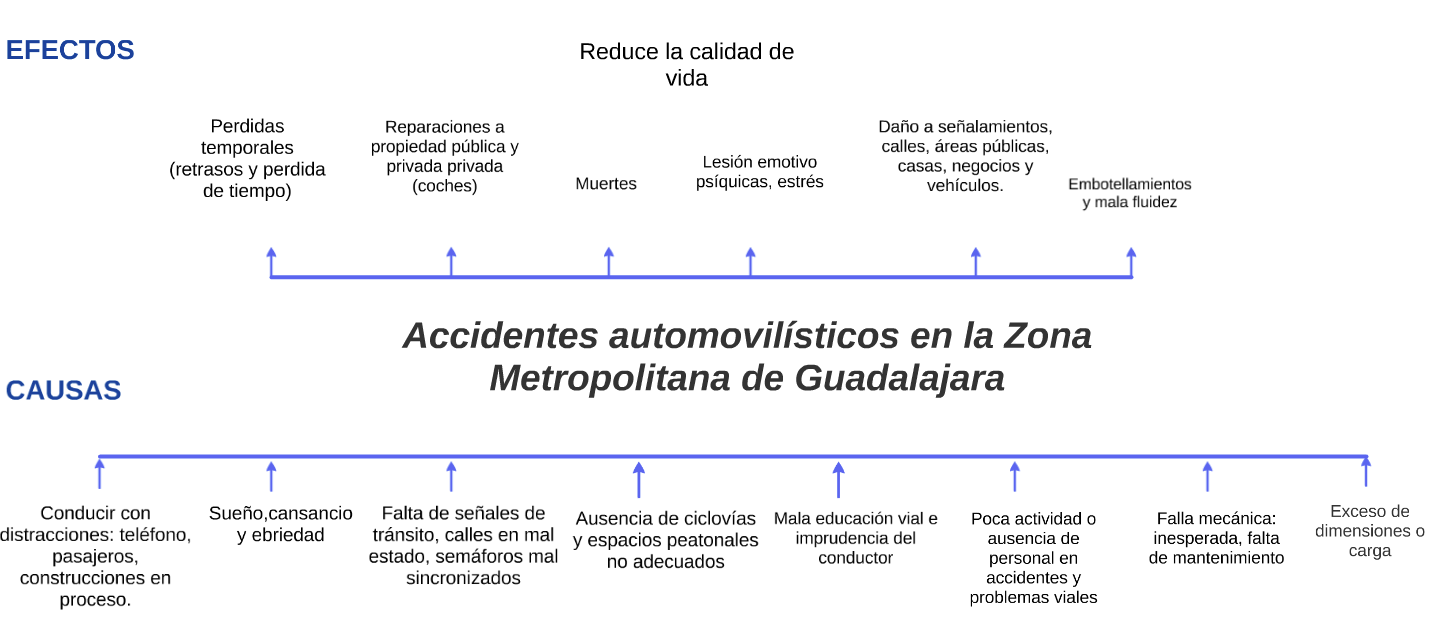
\includegraphics[width=1.25\textwidth]{resources/img/arbol_de_problemas.png}
	\caption{\label{fig:arbol} Árbol de problemas}
    \end{figure}

[agregar contenido]

\section{Objetivos del proyecto}\label{sec:objs}
[agregar contenido]

\subsection{Objetivos general}\label{subsec:general-objs}
[agregar contenido]

\subsection{Objetivos específico}\label{subsec:specific-objs}
[agregar contenido]

\section{Análisis de los participantes}\label{sec:participants}
[agregar contenido]

\section{Alternativas de solución}\label{sec:alternatives}
[agregar contenido]

\section{Elaboración de la MIR}\label{sec:mir}
[agregar contenido]

\section{Conclusiones}\label{sec:conclutions}
[agregar contenido]

\section{Bibliografía}\label{sec:references}
[agregar contenido]

\end{document}
